\subsection{Compartment-based Stochastic Simulation of Diffusion}
\label{stochdiff}
To simulate spatially inhomogeneous chemical systems, the concept of compartments has to be introduced. A compartment $c$ is a subvolume of the the complete domain of interest $V$. The set of all compartments $C$ is a partition of the system domain, i.e.\ $c \cap d = \emptyset \:\forall c,d \in C, c \ne d$ (Compartments don't overlap) and $\bigcup_{c \in C} c = V$ (The complete domain is covered by the compartments). The assumption that only particles close to one another can collide and consequently react is reflected by the principle that only molecules within a compartment can interact. Diffusion, on the other hand, is modeled as a jump process of molecules migrating from a compartment to one of its neighbours. Figure \ref{fig:jumpprocess} illustrates the idea. 

\begin{figure}
\centering
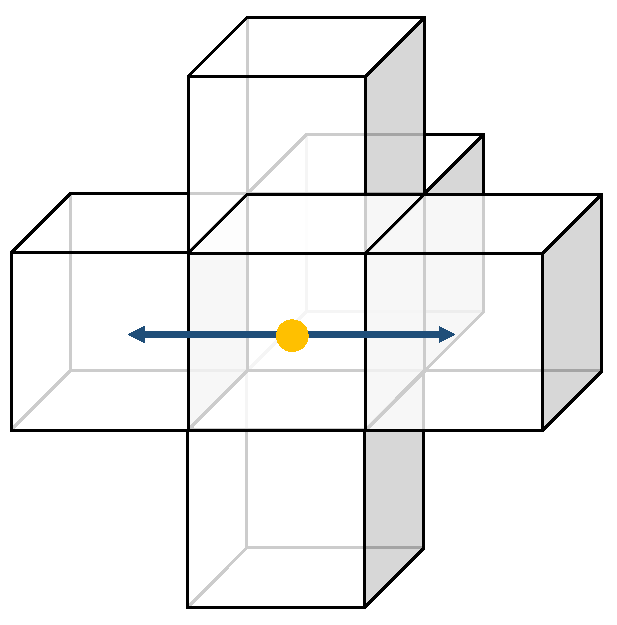
\includegraphics[width=\textwidth]{images/jumpprocess.pdf}
\caption{Illustration of the jump process used to model diffusion in stochastic simulations. The front compartment is omitted for reasons of visual clarity. The arrows indicate two out of six possible directions in which the particle can move. }
\label{fig:jumpprocess}
\end{figure}

In general, the shape of the compartments is arbitrary. In this thesis, however, a cubic domain $\lbrack0,1\rbrack^3$ will be decomposed into $L^3$ uniform cubes with side length $h = 1 / L$. Every compartment is identified by its set of indices $(i,j,k) \in [1,\ldots,L]^3$. The volume in space that is covered by the compartment is $\lbrack (i-1)h,ih\rbrack \times \lbrack (j-1)h,jh \rbrack \times \lbrack (k-1)h,kh \rbrack$. 
By introducing stochastic diffusion constants $d_U$ and $d_V$ a modified description of the Gray-Scott model presented in chapter 2 can be obtained:

\underline{Reactions}
\begin{align}
\label{eq:r1mod}
\cee{\emptyset{} &->[F] U_{i,j,k}} \\
\label{eq:r2mod}
\cee{U_{i,j,k} &->[F] \emptyset} \\
\label{eq:r3mod}
\cee{V_{i,j,k} &->[F+\kappa] \emptyset} \\
\label{eq:r4mod}
\cee{U_{i,j,k} + 2V_{i,j,k} &->[\rho] 3V_{i,j,k}}
\end{align}
with positive reaction rate constants $F$, $\kappa$ and $\rho$.

\underline{Diffusion}
\begin{align}
\label{eq:d1}
\cee{S_{i,j,k} &<->[d_S] S_{i\pm{}1,j,k}} \\
\cee{S_{i,j,k} &<->[d_S] S_{i,j\pm{}1,k}} \\
\cee{S_{i,j,k} &<->[d_S] S_{i,j,k\pm{}1}}
\label{eq:d3}
\end{align}
for the two species $\text{S} \in \{\text{U, V}\}$ with positive diffusion constants $d_\text{U}$ and $d_\text{V}$. The spatial dependency of the system is therefore reflected by the compartment index (i,j,k). It is assumed that only particles within a compartment can  react according to equations \eqref{eq:r1mod} - \eqref{eq:r4mod}. Equations \eqref{eq:d1} - \eqref{eq:d3} describe how particles can migrate from one compartment to another. 

It shall be noted that the chosen discretization approach introduces artificial anisotropy to the system in the sense that the number of directions a particle can move in is not infinite, but limited to 6. Consider, for example, a particle that moves along the vector $\lbrack h,h,0 \rbrack^T$. In reality, the distance the particle travels is $d_r = \sqrt{2}h$, in the discretized model it has to travel $d_d = 2h$. For small $h$, however, this effect can be neglected. Furthermore, the analysis of the possible consequences is beyond the scope of this thesis. 

In order to be able to compare the results of the deterministic and the stochastic approach towards diffusion, it remains to derive a relation between the diffusion parameters in both types of simulation. It is obvious that when the compartment length $h$ is reduced, the diffusion constant has to be increased to keep the "average diffusion velocity" of the particles constant. It has been shown (cite) that deterministic and stochastic simulation are equivalent when $d$ is chosen as
\begin{align}
\label{eq:rescale_diff}
d = \frac{D}{h^2}
\end{align}
An illustrative way to derive this relation is as follows: Considering Fick's law of diffusion $\frac{\partial u}{\partial t} = \Delta u$ and applying a central finite-difference approximation for the Laplace operator leads to:
\begin{equation}
\begin{split}
\Delta u &\approx D\frac{u_{i+1,j,k} + u_{i-1,j,k} + u_{i,j+1,k} + u_{i,j-1,k} + u_{i,j,k+1} + u_{i,j,k-1} - 6u_{i,j,k}}{h^2} \\
&= \frac{D}{h^2}u_{i+1,j,k} + \frac{D}{h^2}u_{i-1,j,k} + \frac{D}{h^2}u_{i,j+1,k} + \frac{D}{h^2}u_{i,j-1,k} + \frac{D}{h^2}u_{i,j,k+1} + \frac{D}{h^2}u_{i,j,k-1} \\
&- 6\frac{D}{h^2}u_{i,j,k}
\end{split}
\end{equation}
It is obvious that this is equivalent to the stochastic approach if $d$ is chosen as in equation \eqref{eq:rescale_diff}. 

Considering the results stated above, it turns out that spatially inhomogeneous systems can be simulated with both the Gillespie and the tau-leaping algorithm without any changes just by applying the compartment approach. However, the resulting system is by far more complex than its spatially homogeneous equivalent (in both, a mathematical and a computational sense). Considering $L^3$ cubic compartments in a three-dimensional cubic domain and a reaction system that consists of $N$ local species subject to $M$ reactions, one has $N L^3$ species and $(M+3N) L^3$ reactions. 

\ifdebug
Reasoning: Molecules must collide before they can react (for 2nd and higher order). $\rightarrow$ reaction within compartment makes sure that molecules are close to each other (have a chance to collide)
\fi